%!TEX program = xelatex
\documentclass{article}

\usepackage[T1]{fontenc}
\usepackage[polish]{babel}
\usepackage[utf8]{inputenc}
\usepackage{titling}
\usepackage{multicol}
\usepackage{paracol}
\usepackage{indentfirst}
\usepackage{float}

\usepackage[letterpaper,top=2cm,bottom=2cm,left=3cm,right=3cm,marginparwidth=1.75cm]{geometry}

\usepackage{amsmath}
\usepackage{graphicx}
\usepackage[colorlinks=true, allcolors=blue]{hyperref}

\begin{document}

\begin{titlepage}
    \begin{center}\LARGE POLITECHNIKA WROCŁAWSKA \\ WYDZIAŁ INFORMATYKI I TELEKOMUNIKACJI \end{center}
    \vspace{57pt}
    \begin{center} \Huge Układy cyfrowe i systemy wbudowane 2 \end{center}
    \vspace{35pt}
    \begin{center} \LARGE Instrument muzyczny \\ Wstępne założenia projektowe \end{center}
    \vspace{50pt}
    \begin{flushleft}\Large Termin zajęć: PON, 8:00-11:00 TP   \end{flushleft}
    \vspace{15pt}
    \begin{paracol}{2}
        \raggedright{\Large Autorzy (Grupa B):} \switchcolumn \raggedleft{\Large Prowadzący zajęcia:} \switchcolumn
        \raggedright{\Large Maciej Byczko, 252747} \switchcolumn \raggedleft{\Large dr inż. Jacek Mazurkiewicz} \switchcolumn
        \raggedright{\Large Bartosz Matysiak, 252757} 
    \end{paracol}
    \vspace{250pt}
    \begin{center}Wrocław, \the\year{}r.\end{center}
\end{titlepage}

%\tableofcontents

\section{Temat projektu}

Projekt ma dotyczyć wykonania emulatora instrumentu muzycznego typu ''keyboard'' z funkcją prostego syntezatora przy użyciu płyty Spartan 3E.

\section{Opis funkcjonalności} % tą sekcję chyba zamienić w zwykły akapit

\subsection{Wersja podstawowa}

\begin{itemize}
    \item Możliwość użycia gamy dźwięków uprzednio nagranych na kartę SD. 
    \item Wsparcie dla klawiatury komputerowej.
    \item Odtworzenie dźwięku.
\end{itemize} 

\subsection{Możliwe rozszerzenia}

\begin{itemize}
    \item Możliwość prostej syntezy jednotonowej.
    \item Wsparcie dla \href{https://pl.wikipedia.org/wiki/Launchpad}{launchpada}.
\end{itemize}

\begin{figure}[H]
    \centering
    \resizebox*{\textwidth}{!}{
        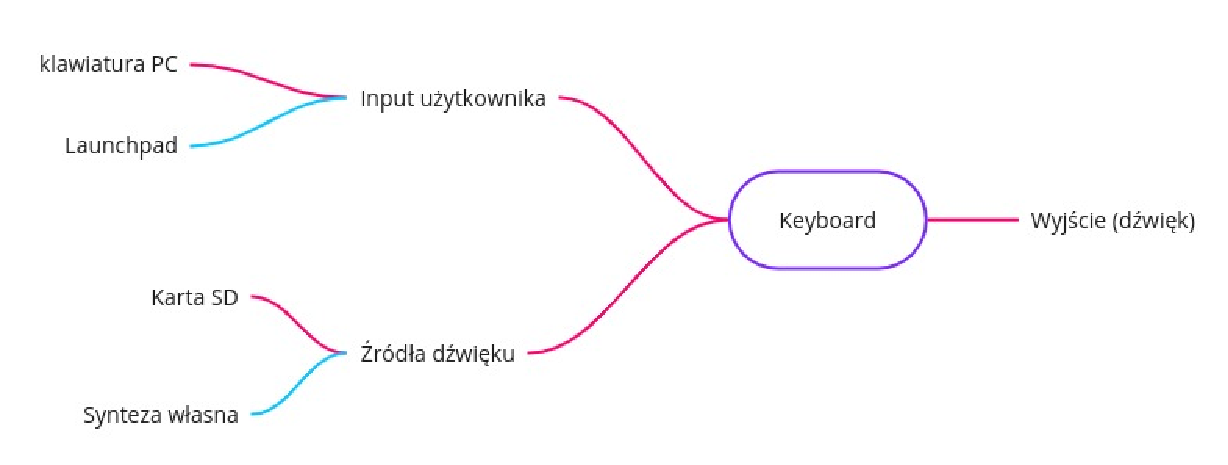
\includegraphics{Mind Map.pdf}
    }
\end{figure}

\section{Podział projektu na moduły}

\subsection{Wykorzystane moduły ze strony kursu}

\begin{itemize}
    \item \textbf{WAVreader} - obsługa karty SD 
    \item \textbf{PS2\_Kbd} lub \textbf{RS232} - obsługa klawiatury PS2 
    \item \textbf{USB\_Function} - obsługa launchpada  % (TO-REVIEW Maciej) tak mi się wydaje, przynajmniej takie pady widziałem
\end{itemize}

\subsection{Moduły własne, przygotowane na potrzeby projektu}

\begin{itemize}
    \item Moduł konwertujący wartości wprowadzone przez użytkownika na odpowiednie wartości tonów dźwięku %strasznie długie, za długie
    \item Moduł do obsługi głośnika % jaki głośnik chcemy? (możliwe, że przyda się też converter DAC: )
\end{itemize}

\end{document}